\documentclass[12pt, twoside]{article}
\usepackage[letterpaper, margin=1in, headsep=0.5in]{geometry}
\usepackage[english]{babel}
\usepackage[utf8]{inputenc}
\usepackage{amsmath}
\usepackage{amsfonts}
\usepackage{amssymb}
\usepackage{tikz}
\usetikzlibrary{quotes, angles}
\usepackage{graphicx}
\usepackage{multicol}

%\usepackage{pgfplots}
%\pgfplotsset{width=10cm,compat=1.9}
%\usepgfplotslibrary{statistics}
%\usepackage{pgfplotstable}
%\usepackage{tkz-fct}
%\usepackage{venndiagram}

\usepackage{fancyhdr}
\pagestyle{fancy}
\fancyhf{}
\renewcommand{\headrulewidth}{0pt} % disable the underline of the header

\fancyhead[RE]{\thepage}
\fancyhead[RO]{\thepage \\ Name: \hspace{3cm}}
\fancyhead[L]{BECA / Dr. Huson / Geometry 10th Grade\\* Unit 4: Parallels and transversals \\ 1 November 2019}

\begin{document}
\subsubsection*{4.11 Exam: Transversals, volume; angle relationships}
  \vspace{0.25cm}
  \begin{enumerate}


  \item Find the area of the parallelogram $ABCD$ shown below, with $AB=11.7$ and height $h=7.5$.
  \begin{flushright}
  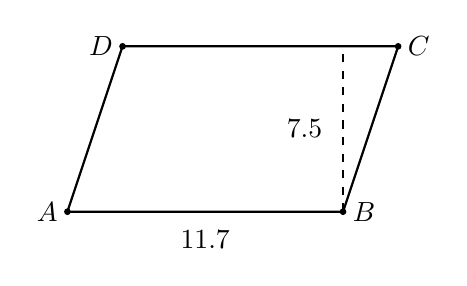
\begin{tikzpicture}[scale=0.7]
    \draw [-, thick] (0,0)--(5,0)--(6,3)--(1,3)--cycle;
    \draw [-, dashed] (5,0)--(5,3);
    \draw [fill] (0,0) circle [radius=0.05] node[left]{$A$};
    \draw [fill] (5,0) circle [radius=0.05] node[right]{$B$};
    \draw [fill] (6,3) circle [radius=0.05] node[right]{$C$};
    \draw [fill] (1,3) circle [radius=0.05] node[left]{$D$};
    \node at (4.3, 1.5){$7.5$};
    \node at (2.5, -0.5){11.7};
  \end{tikzpicture}
  \end{flushright}

  \item Find the sum of the measures of the internal angles of a hexagon. Show the formula.  \vspace{3cm}

  \item  A wooden cutting board is $10 \frac{1}{2}$ inches long, 8 inches wide, and $1 \frac{1}{4}$ inches thick. Find the volume of the box. Show the calculation.
\begin{flushright}
  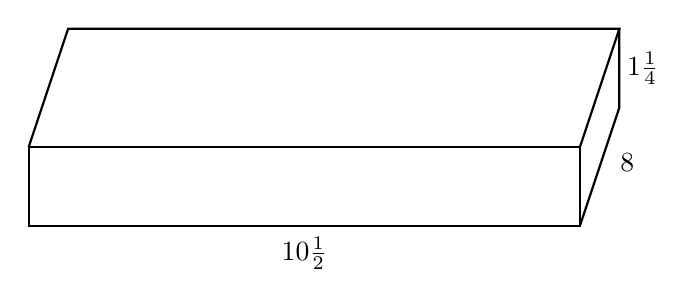
\begin{tikzpicture}[scale=1]
    \draw [-, thick] (0,0)--(7,0)--(7,1)--(0,1)--cycle;
    \draw [-, thick] (0,1)--(0.5,2.5)--(7.5,2.5)--(7,1);
    \draw [-, thick] (7,0)--(7.5,1.5)--(7.5,2.5);
    \node at (7.8, 2){$1 \frac{1}{4}$};
    \node at (3.5, -0.35){$10 \frac{1}{2}$};
    \node at (7.6, 0.8){$8$};
  \end{tikzpicture}
  \end{flushright} \vspace{1cm}

\item Given isosceles $\triangle LMN$ with $\overline{LM} \cong \overline{NM}$. If $m\angle L=2x+20$ and $m\angle N=3x+5$, find $m\angle M$.
\begin{flushright}
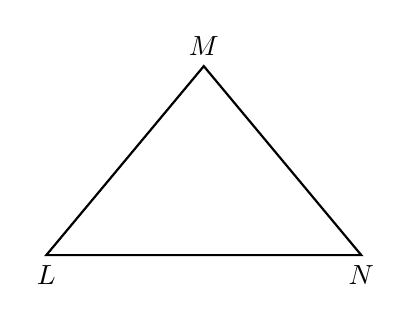
\begin{tikzpicture}[scale=0.8]
  %\draw [->, thick] (0,0)--(5,5);
  \draw [-, thick] (0,0) node[below]{$L$}--
    (2.5,3) node[above]{$M$}--
    (5,0) node[below]{$N$}--cycle;
\end{tikzpicture}
\end{flushright} \vspace{2cm}

\newpage

    
\item Find the area of $\triangle KAT$. The altitude $h$ of the triangle is 11.0 centimeters and the base $KA=19.6$ cm. Show work by writing an equation before making the calculation.
  \begin{flushright}
    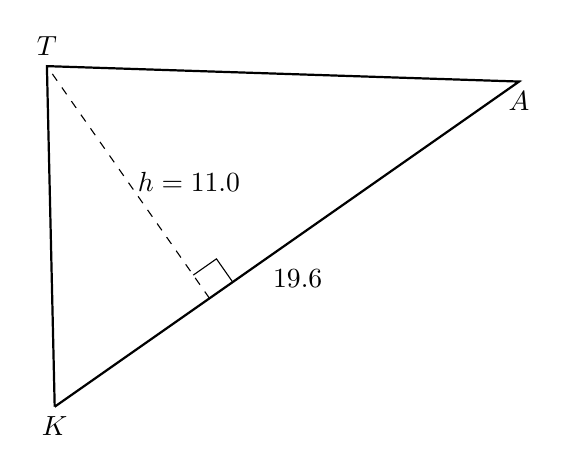
\begin{tikzpicture}[scale=1.2, rotate=35]
      \draw [thick]
        (2,0)node[below]{$K$}--
        (8,0)node[below]{$A$}--
        (4,3)node[above]{$T$} --(2,0);
    \draw [dashed] (4,0)--(4,3);
    \draw (4,0)++(0.3,0)--++(0,0.3)--+(-0.3,0);
    \node at (4,1.5)[right]{$h=11.0$};
    \node at (5,-0.2)[below]{$19.6$};
    \end{tikzpicture} 
  \end{flushright} \vspace{1.0cm}


  \item Construct a line perpendicular to $l$ though $P$.\\
    %\hspace{1cm} Given the line  $l$ and point $P$.
    \vspace{5cm}
    \begin{center}
    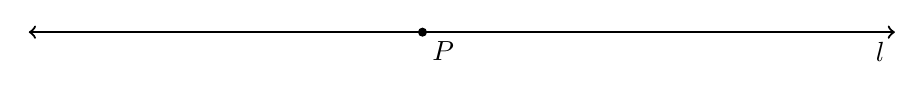
\begin{tikzpicture}
      \draw [<->, thick] (0,0)--(11,0) node[below left]{$l$};
      %\draw [fill] (0,0) circle [radius=0.05] node[left]{$A$};
      %\draw [fill] (11,0) circle [radius=0.05] ;
      \draw [fill] (5,0) circle [radius=0.05] node[below right]{$P$};
    \end{tikzpicture}
  \end{center} \vspace{2cm}

\newpage

  \item Complete the construction of the bisector of the given angle. 
  \vspace{3cm}
    \begin{center}
    \begin{tikzpicture}[rotate=50]
      \draw [<->, thick] (80:7)--(0,0)--(9,0);
      %\draw [fill] (0,0) circle [radius=0.05] node[below]{$A$};
      %\draw [fill] (5,0) circle [radius=0.05] node[below]{$B$};
    \end{tikzpicture}
    \end{center} \vspace{1cm}  

  \item Angles $APC$ and $CPD$ form a linear pair. $m\angle APC = 10x+15$ and $m\angle CPD = 3x-4$. Find $m\angle CPD$. Check your answer for full credit.
  \begin{flushright}
    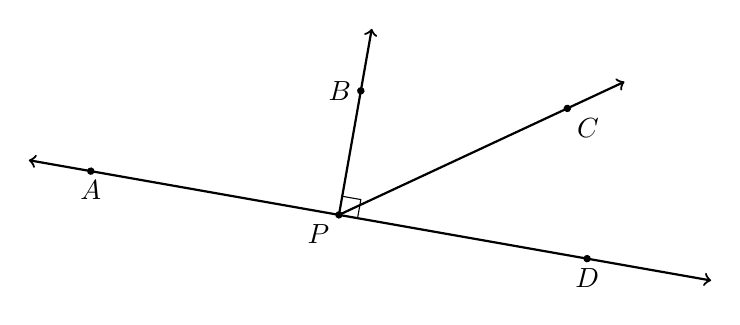
\begin{tikzpicture}[scale=0.8, rotate=-10]
      \draw [->, thick] (0,0)--(35:5);
      \draw [<->, thick] (-5,0)--(6,0);
      \draw [->, thick] (0,0)--(0,3);
      \draw (0,0)++(0.3,0)--++(0,0.3)--+(-0.3,0);
      %\draw [fill] (-1,2.5) circle [radius=0.05] node[left ]{$B$};
      \draw [fill] (35:4) circle [radius=0.05] node[below right]{$C$};
      \draw [fill] (-4,0) circle [radius=0.05] node[below]{$A$};
      \draw [fill] (0,0) circle [radius=0.05] node[below left]{$P$};
      \draw [fill] (0,2) circle [radius=0.05] node[left]{$B$};
      \draw [fill] (4,0) circle [radius=0.05] node[below]{$D$};
    \end{tikzpicture}
    \end{flushright}
    \vspace{5cm}


\newpage

\subsubsection*{Do Not Solve. Circle the appropriate equation, cite a  justification:}
  \begin{multicols}{2}
    \begin{itemize}
      \item ``definition of bisector" 
      \item ``linear pairs sum to $180^\circ$" 
      \item ``vertical $\angle$s are $\cong$" 
      \item ``alternate interior $\angle$s are $\cong$"
      \item ``corresponding $\angle$s of $\parallel$ lines are $\cong$" 
      \item ``same-side interior $\angle$s are supplementary" 
      \item ``$\perp$ rays  with complementary $\angle$s adding to $90^\circ$" 
    \end{itemize}
  \end{multicols}


  \item $\overleftrightarrow{RPU}$ with ray $\overrightarrow{PS}$. \hspace{6cm}
    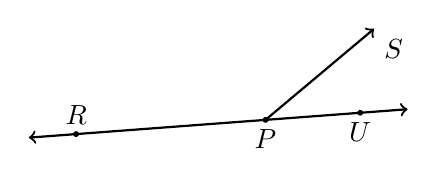
\begin{tikzpicture}[rotate=10, scale=0.6]
      \draw [<->, thick] (-5,.5)--(3,-.3);
      \draw [->, thick] (0,0)--(30:3) node[below right]{$S$};
      \draw [fill] (0,0) circle [radius=0.05] node[below]{$P$};
      \draw [fill] (2,-0.2) circle [radius=0.05] node[below]{$U$};
      \draw [fill] (-4,0.4) circle [radius=0.05] node[above]{$R$};
    \end{tikzpicture}\\[0.5cm]
    $\angle RPS \cong \angle SPU$ \hspace{0.25cm} $m \angle RPS + m \angle SPU = 180^\circ$ \hspace{0.25cm} \rule{6cm}{0.15mm}  \vspace{0.25cm}

    \item Given $m\angle R=m\angle U =65$, and $m\angle UST=130$. Find $m\angle RSU$.
    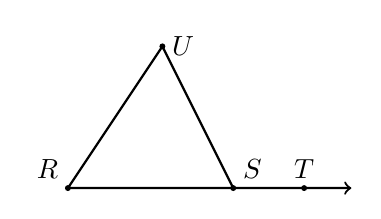
\begin{tikzpicture}[scale=0.6]
      %\draw [->, thick] (0,0)--(5,5);
      \draw [<-, thick] (7,0)--(1,0)--(3,3)--(4.5,0);
      \draw [fill] (1,0) circle [radius=0.05] node[above left]{$R$};
      \draw [fill] (4.5,0) circle [radius=0.05] node[above right]{$S$};
      \draw [fill] (3,3) circle [radius=0.05] node[right]{$U$};
      \draw [fill] (6,0) circle [radius=0.05] node[above]{$T$};
    \end{tikzpicture}\\[0.5cm]
    $\angle UST \cong \angle RSU$ \hspace{0.5cm} $m\angle UST + m\angle RSU =  180$ \hspace{0.5cm} \rule{6cm}{0.15mm} \vspace{0.25cm}

  \item Given $m \angle 1 = 4x+6$, $m \angle 2 = 6x-32$. Find $m \angle 1$.
  \hspace{2cm}
  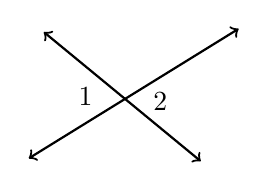
\begin{tikzpicture}[scale=.3, rotate=15]
    \draw [<->, thick] (0,-1.5)--(10,1.5);
    \draw [<->, thick] (2,3.5)--(7,-3.5);
    \node at (3,.4){1};
    \node at (6,-.6){2};
  \end{tikzpicture}\\[0.5cm]
  $\angle 1 \cong \angle 2$ \hspace{1cm} $m\angle 1 + m\angle 2 =  180$ \hspace{0.5cm} \rule{6cm}{0.15mm}
  \vspace{0.5cm}

  \item Given two parallel lines and a transversal, as shown. \hspace{2cm}
  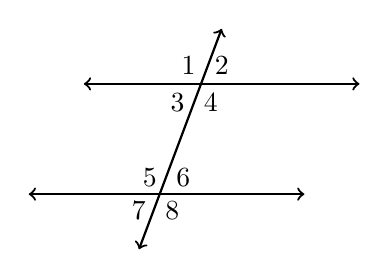
\begin{tikzpicture}[scale=0.7]
    \draw [<->, thick] (3,2)--(8,2);
    \draw [<->, thick] (2,0)--(7,0);
    \draw [<->, thick] (4,-1)--(5.5,3);
    \node at (4.5,0.3) [left]{$5$};
    \node at (4.5,0.3) [right]{$6$};
    \node at (4.3,-0.3) [left]{$7$};
    \node at (4.3,-0.3) [right]{$8$};
    \node at (5.2,2) [above left]{$1$};
    \node at (5.2,2) [above right]{$2$};
    \node at (5,2) [below left]{$3$};
    \node at (5,2) [below right]{$4$};
  \end{tikzpicture} \\[0.5cm]
  $\angle 4 \cong \angle 5$ \hspace{1cm} $m\angle 3 + m\angle 6 =  180$ \hspace{0.5cm} \rule{6cm}{0.15mm}

  \item Given $\overrightarrow{BA} \perp \overrightarrow{BC}$, $m \angle ABD = 2x-5$, and $m \angle DBC = x-10$.
    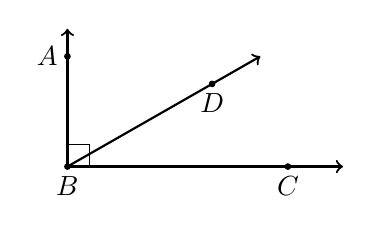
\begin{tikzpicture}[scale=0.7]
      \draw [<->, thick] (0,2.5)--(0,0)--(5,0);
      \draw [->, thick] (0,0)--(3.5, 2);
      \draw [-, thin] (0, 0.4)--(0.4, 0.4)--(0.4, 0);
      \draw [fill] (0,0) circle [radius=0.05] node[below]{$B$};
      \draw [fill] (0,2) circle [radius=0.05] node[left]{$A$};
      \draw [fill] (4,0) circle [radius=0.05] node[below]{$C$};
      \draw [fill] (2.625, 1.5) circle [radius=0.05] node[below]{$D$};
    \end{tikzpicture}\\[0.5cm]
    $\angle ABD \cong \angle DBC$ \hspace{0.5cm} $m\angle ABD + m\angle DBC =  90$ \hspace{0.5cm} \rule{6cm}{0.15mm}

\newpage
\item The measures in degrees of the three angles of a triangle are $3x$, $\frac{1}{2}x+7$, and $5x-65$. Find $x$. \vspace{4cm}

\item Given isosceles $\triangle RSU$ with $\overline{UR} \cong \overline{US}$. If $m\angle UST=x$ and $m\angle R=x-80$, find $m\angle U$.
\begin{flushright}
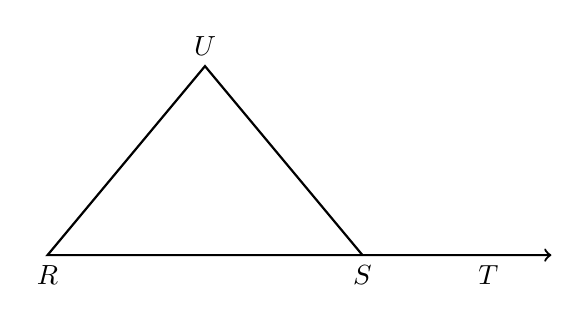
\begin{tikzpicture}[scale=0.8]
  %\draw [->, thick] (0,0)--(5,5);
  \draw [<-, thick] (8,0)--
    (7,0) node[below]{$T$}--
    (0,0) node[below]{$R$}--
    (2.5,3) node[above]{$U$}--
    (5,0) node[below]{$S$};
\end{tikzpicture}
\end{flushright} \vspace{2cm}

\item An angle bisector is shown below, with $\overrightarrow{AC}$ bisecting $\angle BAD$. Given $m\angle BAC = 3x+5$ and $m\angle BAD = 7x-1$, find $m\angle BAD$. (Show check)
\begin{flushright}
\begin{tikzpicture}[scale=0.7, rotate=20]
  \draw [<->, thick] (80:7)node[left]{$B$} 
  --(0,0)node[below]{$A$}
  --(6,0)node[below]{$D$}--(7,0);
  \draw [->, thick] (0,0)--(40:7)node[below right]{$C$};
  %\draw [fill] (0,0) circle [radius=0.05] node[below]{$A$};
  %\draw [fill] (5,0) circle [radius=0.05] node[below]{$B$};
\end{tikzpicture}
\end{flushright} \vspace{2cm}

\newpage

\item Given $\overleftrightarrow{RS}$ as shown on the number line, with $R=-3.3$ and $S=5.1$. \\[20pt] % Midpoint
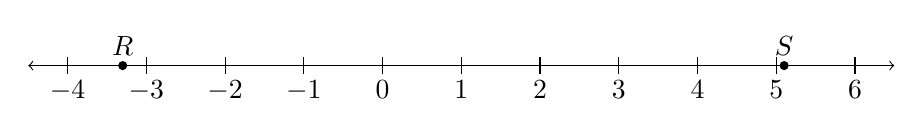
\begin{tikzpicture}
  \draw [<->] (-4.5,0)--(6.5,0);
  \foreach \x in {-4,...,6} %2 leading for diff!=1
    \draw[shift={(\x,0)},color=black] (0pt,-3pt) -- (0pt,3pt) node[below=5pt]  {$\x$};
    \draw [fill] (-3.3,0) circle [radius=0.05] node[above] {$R$};
    \draw [fill] (5.1,0) circle [radius=0.05] node[above] {$S$};
\end{tikzpicture}
\begin{enumerate}
  \item What is the exact distance on the number line between the points $R$ and $S$? \vspace{3cm} 
  \item The point $T$ bisects $\overline{RS}$. Find the value of $T$, and mark and label it on the numberline $\overleftrightarrow{RS}$ shown above. 
\end{enumerate} \vspace{3cm} 


  \item The circle $O$ is shown below with diameter $\overline{AOC}$ and radius $\overline{BO}$. It is given that $m\angle BAO = 62^\circ$. Find the measure of the central angle $\angle AOB$.
  \begin{flushright}
  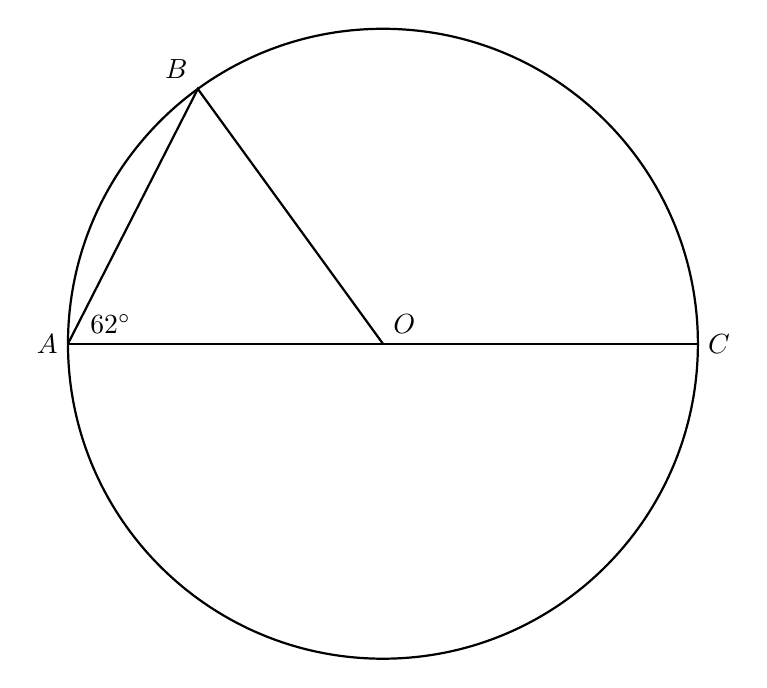
\begin{tikzpicture}[scale=0.8]
    \draw [thick] (0,0) circle [radius=5];
    \draw [-, thick] (-5,0) node[left]{$A$}--
    (0,0) node[above right]{$O$}--
    (5,0) node[right]{$C$};
    \draw [-, thick] (0,0)--(126:5) node[above left]{$B$}--(-5,0);
    \node at (-4.8, 0)[above right]{$62^\circ$};
  \end{tikzpicture}
  \end{flushright} \vspace{2cm}

\newpage
  \item Given isosceles right $\triangle ABC$ with $\overline{AC} \cong \overline{BC}$ and $\overline{AC} \perp \overline{BC}$. Find $m\angle A$.
  \begin{flushright}
  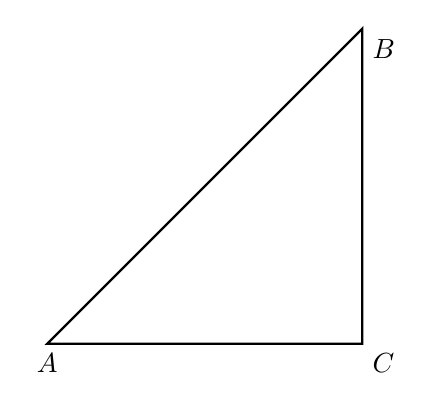
\begin{tikzpicture}[scale=0.5]
    \draw [thick](0,0) node[below]{$A$}--
    (8,0) node[below right]{$C$}--
    (8,8) node[below right]{$B$} --cycle;
  \end{tikzpicture}
  \end{flushright}  \vspace{0.5cm}
   
  \item A sheet metal part is cut with square corners and two $45^\circ$ cutouts as shown with lengths marked in centimeters.
  \begin{enumerate}
    \item Find the area of the figure. (the drawing is not to scale)
      \begin{flushright}
      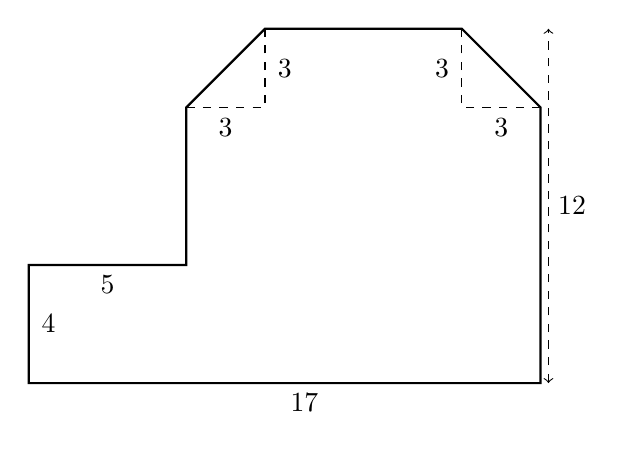
\begin{tikzpicture}[scale=0.5]
        \draw [-, thick] (0,0)--(13,0)--(13,7)--(11,9)--
        (6,9)--(4,7)--(4,3)--(0,3)--cycle;
        \draw [dashed] (4,7)--(6,7)--(6,9);
        \draw [dashed] (13,7)--(11,7)--(11,9);
        \draw [<->, dashed] (13.2,0)--(13.2,9);
        \node at (6.5, 8){3};
        \node at (5, 6.5){3};
        \node at (0.5, 1.5){4};
        \node at (2, 2.5){5};
        \node at (10.5, 8){3};
        \node at (12, 6.5){3};
        \node at (7, -0.5){17};
        \node at (13.8, 4.5){12};
        %\node at (13.5, 8){2};
      \end{tikzpicture}
      \end{flushright} \vspace{3cm}
    \item Spicy: The weight of the sheet metal is 2.25 grams per square centimeter. Find the weight of the part.
  \end{enumerate}

\newpage

  \item The trapezoid $ABCD$ has two parallel sides, $\overline{AB} \parallel \overline{CD}$ with lengths $AB=9$ and $CD=11$. The trapezoid's height is $h=7.25$. Find the area of the trapezoid. \\[0.25cm]
    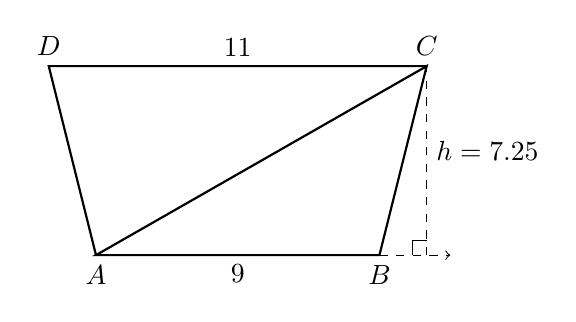
\begin{tikzpicture}[scale=0.6]
      \draw [thick]
        (0,0)node[below]{$A$}--
        (6,0)node[below]{$B$}--
        (7,4)node[above]{$C$} --cycle;
      \draw [thick] (0,0)--(-1,4)node[above]{$D$}--(7,4);
      \draw [dashed] (7,0)--(7,4);
      \draw [dashed, ->] (6,0)--(7.5,0);
      \draw (7,0)++(-0.3,0)--++(0,0.3)--+(0.3,0);
      \node at (7,2.2)[right]{$h=7.25$};
      \node at (3,0)[below]{$9$};
      \node at (3,4)[above]{$11$};
    \end{tikzpicture} \vspace{2cm}

  \item Given parallel lines $\overleftrightarrow{AB} \parallel \overleftrightarrow{CDE}$ with $\overline{AC} \cong \overline{CD}$. If $m\angle BAD=63$ find $m\angle ACD$.
  \begin{flushright}
  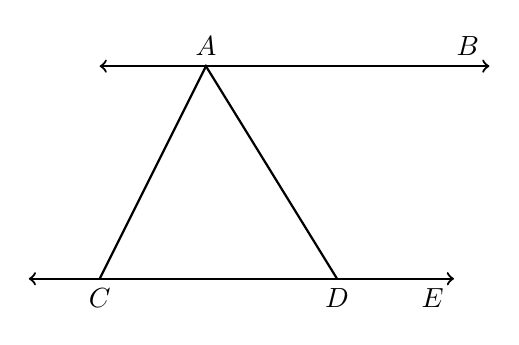
\begin{tikzpicture}[scale=0.9]
    \draw [<->, thick] (1,3)--(6.5,3) node[above left]{$B$};
    \draw [<->, thick] (0,0)--
      (5,0)--
      (6,0) node[below left]{$E$};
    \draw [-, thick] (1,0) node[below]{$C$}--
      (2.5,3) node[above]{$A$}--
      (4.35,0) node[below]{$D$};
  \end{tikzpicture}
  \end{flushright} \vspace{1cm}

  \item Two parallel lines intersect a second set of parallel lines. Given $m\angle 2 = 2.8x+9$ and $m\angle 4 = 4.4x - 63$, find the measure of $\angle 1$. 
    \begin{flushright}
      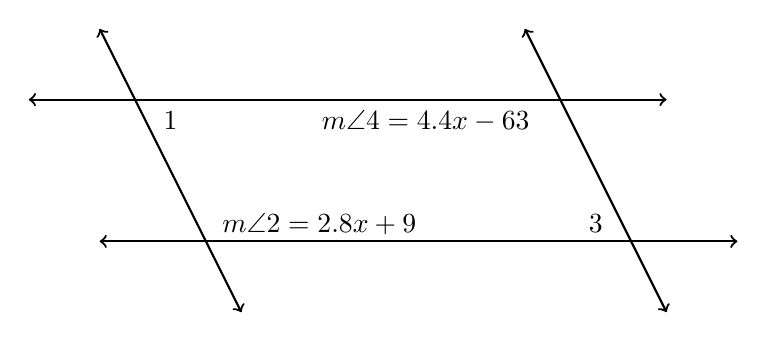
\begin{tikzpicture}[scale=0.9]
        \draw [<->, thick] (3,0)--(12,0);
        \draw [<->, thick] (2,2)--(11,2);
        \draw [<->, thick] (5,-1)--(3,3);
        \draw [<->, thick] (11,-1)--(9,3);
        \node at (4, 1.7){$1$};
        \node at (6.1, 0.25){$m\angle 2 = 2.8x+9$};
        \node at (10, 0.25){$3$};
        \node at (7.6, 1.7){$m\angle 4 = 4.4x - 63$};
      \end{tikzpicture}
      \end{flushright}

\newpage

\subsubsection*{Do Not Solve! \\
Model the situation with an equation in terms of $x$.}

  \item Given $\overline{ABC}$, with $AB=2x-1$, $BC=3x+7$, and $AC=21$. Find $x$. \vspace{1cm}
  \begin{flushright}
    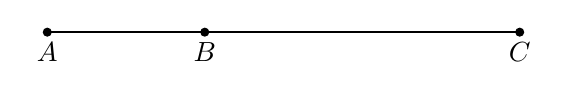
\begin{tikzpicture}
      \draw [-, thick] (0,0) node[below]{$A$}--
      (2,0) node[below]{$B$}--
      (6,0) node[below]{$C$};
      \draw [fill] (0,0) circle [radius=0.05];
      \draw [fill] (2,0) circle [radius=0.05];
      \draw [fill] (6,0) circle [radius=0.05];
    \end{tikzpicture}
    \end{flushright} \vspace{1cm}
  
  \item Given $m\angle 3 = x+35$ and $m\angle 5 = 4x-25$. Find $x$. 
  \begin{flushright}
  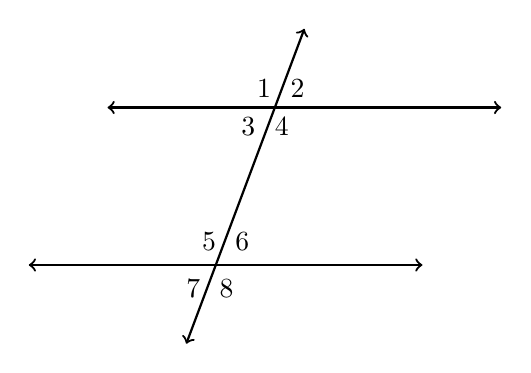
\begin{tikzpicture}
    \draw [<->, thick] (3,2)--(8,2);
    \draw [<->, thick] (2,0)--(7,0);
    \draw [<->, thick] (4,-1)--(5.5,3);
    \node at (4.5,0.3) [left]{$5$};
    \node at (4.5,0.3) [right]{$6$};
    \node at (4.3,-0.3) [left]{$7$};
    \node at (4.3,-0.3) [right]{$8$};
    \node at (5.2,2) [above left]{$1$};
    \node at (5.2,2) [above right]{$2$};
    \node at (5,2) [below left]{$3$};
    \node at (5,2) [below right]{$4$};
  \end{tikzpicture}
  \end{flushright} \vspace{0.5cm}

  \item In the diagram below $m\angle AOB = 6x+5$ and $m\angle COB = 8x+15$. Find $x$. %\vspace{0.25cm}
  \begin{flushright}
  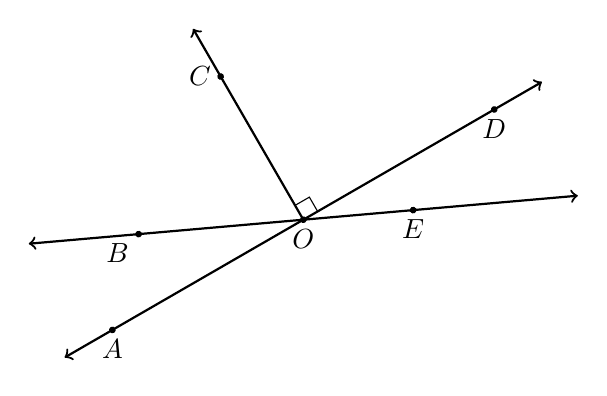
\begin{tikzpicture}[scale=0.7, rotate=30]
  \draw [<->, thick] (-25:5)--(0,0)--(155:5);
  \draw [<->, thick] (-5,0)--(5,0);
  \draw [->, thick] (0,0)--(0,4);
  \draw (0,0)++(0.3,0)--++(0,0.3)--+(-0.3,0);
  %\draw [fill] (-1,2.5) circle [radius=0.05] node[left ]{$B$};
  \draw [fill] (155:3) circle [radius=0.05] node[below left]{$B$};
  \draw [fill] (-4,0) circle [radius=0.05] node[below]{$A$}; 
  \draw [fill] (0,0) circle [radius=0.05] node[below]{$O$};
  \draw [fill] (0,3) circle [radius=0.05] node[left]{$C$};
  \draw [fill] (4,0) circle [radius=0.05] node[below]{$D$};
  \draw [fill] (-25:2) circle [radius=0.05] node[below]{$E$};
  \end{tikzpicture}
  \end{flushright}

  \item The point $K$ is the midpoint of $\overline{JL}$, $JK=3x+15$, and $JL=9x+9$. Find $x$.  \vspace{1cm}
  \begin{flushright}
    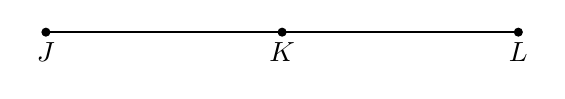
\begin{tikzpicture}
      \draw [-, thick] (0,0) node[below]{$J$}--
      (3,0) node[below]{$K$}--
      (6,0) node[below]{$L$};
      \draw [fill] (0,0) circle [radius=0.05];
      \draw [fill] (3,0) circle [radius=0.05];
      \draw [fill] (6,0) circle [radius=0.05];
    \end{tikzpicture}
    \end{flushright} \vspace{2cm}

\newpage

  \item A feeding trough in the shape of a rectangular prism is 105 inches long. The trough's cross section is square. If its volume is 15,120 cubic inches, what is the dimension of each side of its square end, $x$? (drawing not to scale)
  \begin{flushright}
    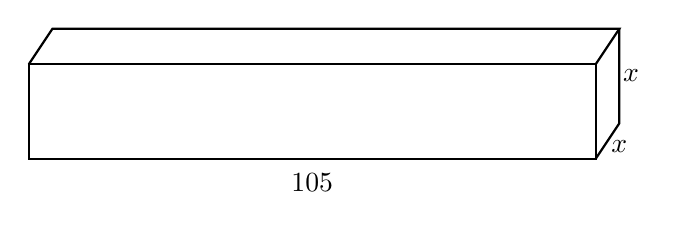
\begin{tikzpicture}[scale=.6]
      \draw [-, thick] (0,0)--(12,0)--(12,2)--(0,2)--cycle;
      \draw [-, thick] (0,2)--(0.5,2.75)--(12.5,2.75)--(12,2);
      \draw [-, thick] (12,0)--(12.5,0.75)--(12.5,2.75);
      \node at (12.75, 1.75){$x$};
      \node at (6, -0.5){$105$};
      \node at (12.5, 0.25){$x$};
    \end{tikzpicture}
    \end{flushright} \vspace{5cm}

  \item Given $\overrightarrow{BA} \perp \overrightarrow{BC}$, $m \angle ABD = 2x$, and $m \angle DBC = x-15$. Find $m \angle DBC$. \\[0.25cm]
  For full credit, show the check using both angle measures.
    \begin{flushright}
    \begin{tikzpicture}[scale=1.2]
      \draw [<->, thick] (0,3) node[left]{$A$}--
        (0,0) node[below]{$B$}--
        (4,0) node[below]{$C$};
      \draw [->, thick] (0,0)--(20:3.5) node[above left]{$D$};
      \draw [-, thin] (0, 0.4)--(0.4, 0.4)--(0.4, 0);
    \end{tikzpicture}
    \end{flushright}
    \vspace{1cm}

\newpage
\subsubsection*{Early finishers}

  \item In the diagram below $m\angle AOB = 3x+11$ and $m\angle DOE = 5x-3$. Find $m\angle DOE$.\\[0.25cm]
  (Calculate $m\angle AOB$ as a check)
  \begin{flushright}
  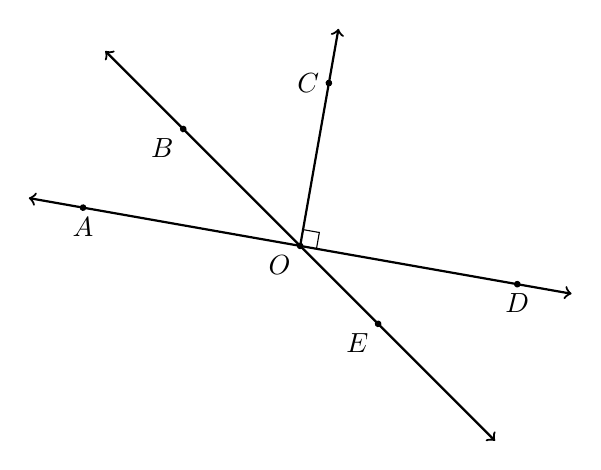
\begin{tikzpicture}[scale=0.7, rotate=-10]
    \draw [<->, thick] (-35:5)--(0,0)--(145:5);
    \draw [<->, thick] (-5,0)--(5,0);
    \draw [->, thick] (0,0)--(0,4);
    \draw (0,0)++(0.3,0)--++(0,0.3)--+(-0.3,0);
    %\draw [fill] (-1,2.5) circle [radius=0.05] node[left ]{$B$};
    \draw [fill] (145:3) circle [radius=0.05] node[below left]{$B$};
    \draw [fill] (-4,0) circle [radius=0.05] node[below]{$A$}; 
    \draw [fill] (0,0) circle [radius=0.05] node[below left]{$O$};
    \draw [fill] (0,3) circle [radius=0.05] node[left]{$C$};
    \draw [fill] (4,0) circle [radius=0.05] node[below]{$D$};
    \draw [fill] (-35:2) circle [radius=0.05] node[below left]{$E$};
  \end{tikzpicture}
  \end{flushright}

  \item One side of the $\triangle ABC$ has a height $h = 11.5$. The triangle's area is 103.5. Find the length of the side $\overline{AB}$.
    \begin{flushright}
      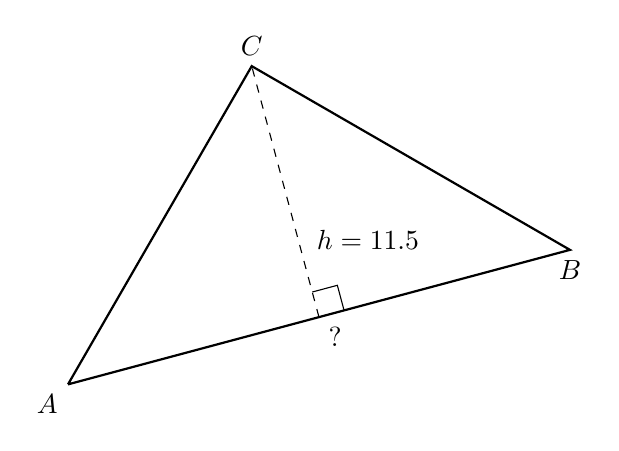
\begin{tikzpicture}[scale=1.1, rotate=15]
      \draw [thick]
        (2,0)node[below left]{$A$}--
        (8,0)node[below]{$B$}--
        (5,3)node[above]{$C$} --(2,0);
      \draw [dashed] (5,0)--(5,3);
      \draw (5,0)++(0.3,0)--++(0,0.3)--+(-0.3,0);
      \node at (5.1,0.9)[right]{$h = 11.5$};
      \node at (5,0)[below right]{?};
      \end{tikzpicture} \vspace{1.0cm}
  \end{flushright}

  \item Of two complementary angles, the measure of $\angle A$ is five times that of $\angle B$. Find $m\angle A$. \vspace{3.5cm} 


\newpage

  \item Given parallel lines $\overleftrightarrow{AB} \parallel \overleftrightarrow{CDE}$ with $\overline{AD} \cong \overline{CD}$. If $m\angle 1=78$ find $m\angle 2$.
  \begin{flushright}
  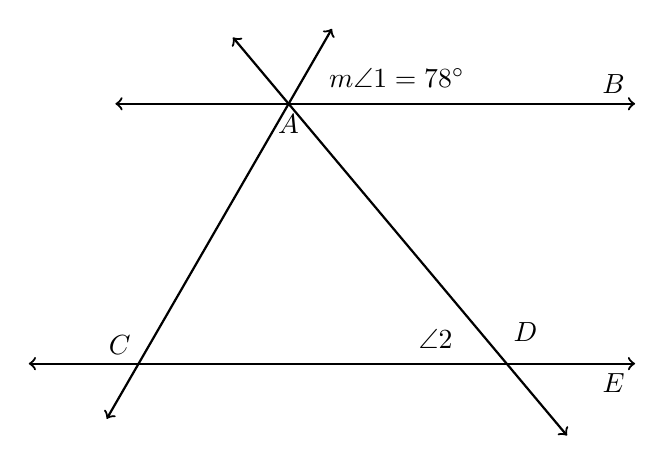
\begin{tikzpicture}[scale=1.1]
    \draw [<->, thick] (-2,0)--(4,0) node[above left]{$B$};
    \draw [<->, thick] (-3,-3)--
      (4,-3) node[below left]{$E$};
    \draw [<->, thick] (-120:4.2)--
      (0,0) node[below]{$A$}--(60:1);
    \draw [<->, thick] (130:1)--(-50:5);
    \node at (1.25, 0.3){$m\angle 1=78^\circ$};
    \node at (-44:3.8){$D$};
    \node at (-125:3.4){$C$};
    \node at (-58:3.2){$\angle 2$};
  \end{tikzpicture}
  \end{flushright} \vspace{4cm}

  \item The volume of the rectanglar prism shown is 120 cubic feet. Its length is length is ten feet longer than its height $x$. Its depth is 5 feet. Find the length of the prism. \\(not drawn to scale)
  \begin{flushright}
    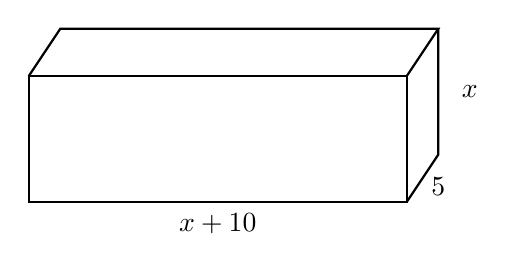
\begin{tikzpicture}[scale=0.8]
      \draw [-, thick] (0,0)--(6,0)--(6,2)--(0,2)--cycle;
      \draw [-, thick] (0,2)--(0.5,2.75)--(6.5,2.75)--(6,2);
      \draw [-, thick] (6,0)--(6.5,0.75)--(6.5,2.75);
      \node at (7, 1.75){$x$};
      \node at (3, -0.35){$x+10$};
      \node at (6.5, 0.25){$5$};
    \end{tikzpicture}
    \end{flushright} \vspace{3cm} 


  \end{enumerate}
\end{document}
